\documentclass{article}

\usepackage[hyphens]{url}
\usepackage{fontspec}
\usepackage{graphicx}

\graphicspath{ {./images/} }

\defaultfontfeatures{Mapping=tex-text,Scale=1.00}
\setmainfont{Inter Light}
\setmonofont{Liberation Mono}
% \usepackage[sfdefault,light]{inter} % this needs tex live
% \usepackage[T1]{fontenc}
\linespread{1.50}
\sloppy

\begin{document}
\title{The Craft of Code: Practice and Knowledge in the Production of Software}
\author{Pierre Depaz}
\date{January 2021}
\maketitle

\section{Introduction}

Code has often been examined through computation\cite{berry_philosophy_2011}, humanities \cite{hayles_my_2010}, or social sciences\cite{mackenzie_cutting_2006}, rather than as a result of the practice of programming. This article proposes to investigate the specificities of writing code within the tradition of craftsmanship. Indeed, code is a myriad of socio-technical \textit{assemblages} composed of programming languages, operating systems and tools. These in turn exist within a cultural context made up of stories and texts, both from academic and folk origins. This article relies on a shift from an abstract conception of code, to one in which a variety of actors\cite{hayes_cultures_2017}, self-identifications and narratives from programmers themselves is put at the forefront. The main distinction we start with is between the theoretical computer scientist, and the practical software developer, focused on writing and reading code.

Links between craftsmanship and programming have existed as self-proclaimed ones by programmers themselves, as well as by academics \cite{sennett_craftsman_2009}, but have not yet been elucidated under specific angles. Michel De Certeau describes the concept of \textit{tactics}, bottom-up actions designed and implemented by the users of a situation, product or technology as opposed to \textit{strategies}\cite{certeau_invention_1990}, in which ways of doing are prescribed in a top-down fashion. It is two of these tactics that we investigate here---knowledge and beauty in programming.

To do so, we start from a parallel with medieval architecture, then move on to the place of implicit knowledge in process of programmers learning their craft, and conclude on the reality of code as a material. These incursions in programming as craftsmanship conclude on the possibility of a specific craft of the twenty-first century.

\section{Parallels}

\subsection{Craftsmanship through the ages}

Craftsmanship is often seen as that which was \emph{before} manufacture, and as \emph{tool-based, intrinsically-motivated work which produces functional artefacts}\cite{sennett_craftsman_2009}. It stood out in the late Middle-Ages through their socio-economic organization, and their relationship to knowledge. Organized in guilds, they exhibited strong cohesion: between a master and their apprentices, and between equal practicioners\cite{black_guilds_1984,wolek_managerial_1999}.

While crafts included glossaries to describe the details of their trade\cite{bassett_craftsman_2008}, the standards for quality were less explicit. Cennino Cennini, in his \emph{Libro dell'arte}, one of the first codexes to map out craft knowledge in the early Renaissance, lays out practical advice on specific painting techniques, but does not explicitly mention how to make something \emph{good}\cite{cennini_craftsmans_2012} and further attempts, at the eve of the Industrial Revolution, continued this formalization\cite{pannabecker_diderot_1994}, resulting into being integrated with modern industrial processes\cite{gordon_who_1988,mcgee_craftsmanship_1999}.

\subsection{Programmers as craftsmen}

Early computer enthusiasts described as hackers developed organizational features similar to their historical counterparts: spread in different geographic locations (Stanford, MIT, Bell Labs)\cite{raymond_cathedral_2001}, emphasis was put on engagement with tools\cite{stephenson_beginningwas_1999}, inquiring into peers' work\cite{levy_hackers_2010} and later formalized into bottom-up archives\footnote{The most famous of which is the Jargon File, later to be published as the The New Hacker's Dictionary: \url{http://www.catb.org/jargon/html/}}. Little accountability was required when it came to design explicitness: both the UNIX operating system and the TCP/IP protocol were originally realized without overarching supervision or extensive documentation\cite{seibel_coders_2009,raymond_cathedral_2001}.

As computer science solidified as a distinct field in the 1960s, there was a process of formalizing the hitherto \textit{ad hoc} techniques of programming computers. As a response to the myth of carefully hand-made code\footnote{See The Story of Mel, A Real Programmer, a folktale of early programmers: \url{https://www.cs.utah.edu/~elb/folklore/mel.html}} and free-form programming came the structured programming approach\cite{dijkstra_chapter_1972}. With the operating system and the personal computer revolutions, access to tools became widespread, and transformed tightl communities into a global network of exchange. Inquiries into the relationship of craftsmanship with programming started to take place in the mid-1970s from educational\cite{dijkstra_craftsman_1982}, organizational\cite{brooks_mythical_1975} and inter-personal perspectives\cite{weinberg_psychology_1998}, and culminated with the publication of several trade books\cite{martin_clean_2008,hendrickson_software_2002}, explicitly connecting the craft of programming with previous craft activities, and emphasizing the need for intrinsic motivation and the aim of a job well-done\cite{hoover_apprenticeship_2009,goodliffe_code_2007}, rather than passive execution\footnote{See code monkey: \url{http://www.techopedia.com/definition/31469/code-monkey}}.

\subsection{The case of architecture}

A counterpart to the computer scientist is the classical architect, but in an inverse relation: the architect emerged from centuries of hands-on work\cite{pevsner_term_1942}, while the computer scientist was first to a field of practicioners, followed by a need to regulate and structure those practices. Different sequences of events, perhaps, yet mirroring each other. On one side, construction work without an explicit architect, under the supervision of bishops and clerks, did indeed lead to significant results (e.g. Notre Dame de Paris, Basilica of Sienna). On the other side, letting go of structured and restricted modes of working characterizing computer programming up to the 1980s was described in \textit{The Cathedral and the Bazaar}. Discussing the Linux project and its open-source philosophy, it showed how the quantity of self-motivated workers without rigid structures can result in better work than if made by a few, highly-skilled individuals\cite{raymond_cathedral_2001}.

In both cases, cooperation on a long-term basis out of intrinsic motivation, and without clear, individual ownership of the result, is possible; a parallel echoed in the similar concepts of \textit{collective craftsmanship} in the Middle-Ages and the \emph{egoless programming} of today\cite{brooks_mythical_1975}.

\section{Acquiring knowledge}

\subsection{Bus factor and tacit knowledge}

The problem of knowledge in programming can be examplified by the "bus factor"\footnote{\url{https://en.wikipedia.org/w/index.php?title=Bus_factor}}. It describes the risk of crucial information being lost due to the disappearance or incapacity of one of the programmers of the project. Given the \emph{essential complexity}\footnote{See the \textit{No Silver Bullet} essay in \emph{The Mythical Man-Month}, op.cit.} of programming, along with the compulsive behaviours sometimes exhibited by intrinsically motivated programmers\cite{weizenbaum_computer_1976}, the gap between design and implementation---the domain of the craftsman---often relies on tacit knowledge\cite{collins_tacit_2010}.

Explicit knowledge, in programming as in most disciplines, is carried through books, academic programs and, more recently, web-based content, but both seem insufficient to reach an expert level\cite{davies_models_1993}. Without tacit knowledge, the road to good code is quite unclear.

\begin{figure}
    \centering
    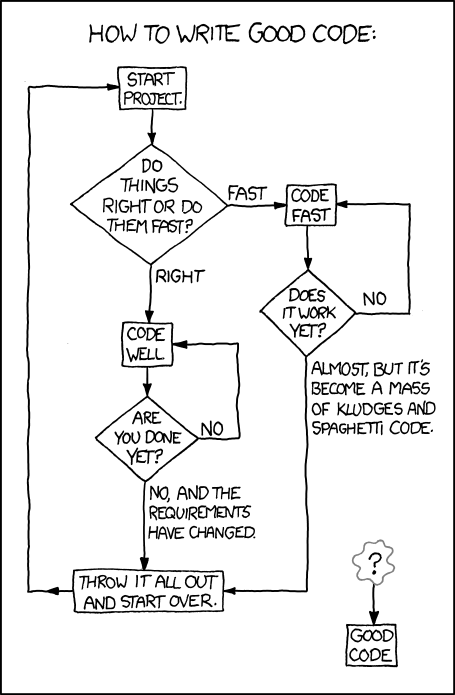
\includegraphics[scale=0.5]{good_code.png}
    \caption{Source: https://xkcd.com/844/}
\end{figure}


\subsection{Apprentices and masters}

The acquisition of such implicit knowledge in craftsmanship takes place through the apprentice-master relationship, and the act of copying. In the former, a learner starts by imitating the way of working of the master, where important aspects of the craft are being demonstrated to the apprentice by a more experienced practicioner, rather than formalized and learned independently. Sometimes, this relationship to a master is explicit via practices such as pair programming\cite{williams_pair_2003} or corporate mentorship (IBM's Master programmer initiative). Other times, it is re-interpretated through fictional accounts designed to impart wisdom on the readers, and taking inspiration from Taoism and Zen\cite{james_tao_1987}. This sort of informal teaching by showing has been implemented in various languages as a practical learning experience\footnote{See, for instance: \url{http://rubykoans.com/}}. Without the presence of an actual master, the programming apprentice takes the program writer as their master to achieve each of the assigned tasks. The role historically given to the master craftsman is delegated into the code itself, containing both the problem and the solution, straddling the line between formal exercises and interactive practice.

Code's ability to be copied complicates the argument of software as craftsmanship in terms of knowledge transmission. Since craftsmanship has been understood as that which is done by hand, and since craftsmen were working with unique artefacts (i.e. no artefact can be perfectly copied), copying someone else's realization was physically inconceivable. The realm of software, on the opposite, relies on the technical affordance of code to be seamlessly duplicated\cite{manovich_language_2001}. This lets anyone inspect and use code, but even though the ability to perfectly copy anyone else's work became widely available to programmers, the difference between amateur and expert programmers lie in the extent to which they indeed blindly copy, or draw inspiration to write their own\cite{treude_understanding_2017}\footnote{See the discussions on \url{https://softwareengineering.stackexchange.com/questions/36978}}.

Eastern craftsmanship further qualify these different approaches to copying. \emph{Moxie}, a Chinese term for copying and practice, is a key concept in how an apprentice can equal their master through thougtful replication \cite{man_influence_2015,jordan_copying_2003}---manually copying from quality work to seize their elusive essence is an essential aspect to craftsmanship.

\subsection{The problem with copying}

So while programmers are to acquire implicit knowledge through a process of learning by doing, we need to assess how much of it happens through observing. Implied in the apprentice-master relationship is that what is observed should be of \textit{good quality}; one learns through ones own mistakes, and through seeing examples of good work. Coming back to the relationship between architecture and software development, Christopher Alexander asks, in the preface of Richard P. Gabriel's \textit{Patterns of Software}\cite{gabriel_patterns_1998},

\begin{quote}
    \textit{For a programmer, what is a comparable goal? What is the Chartres of programming? What task is at a high enough level to inspire people writing programs, to reach for the stars?}
\end{quote}

If a craftsman learns their trade by comparing their work with work of a higher quality, the programmer faces a problem: a lot of examples, but a few good ones\cite{taylor_patterns_2001}: copyright stands in the way of pedagogical copying. With software becoming protectable under copyright laws in the 1980s\cite{oman_computer_2018}, great works of programming craft became unacessible to programmers, despite their knowledge-value\cite{gabriel_mob_2001}. One of the most famous examples is \emph{Lions' Commentary on UNIX 6th Edition, with Source Code}, which was circulated illegaly in classrooms for twenty years before its official publication was authorized by the copyright owners\cite{lions_lions_1996}.

\section{Material aesthetics}

Complementing this process of knowledge acquisition is the \emph{practice} of programming, and inherent in the practice is the \emph{good practice}, the one leading to a beautiful result.

\subsection{The beauty of a thing well-made}

A traditional perspective is that of the motor skills, with dexterity, care and experience as essential features of a craftsman's ability to realize something beautiful\cite{osborne_aesthetic_1977}, along with self-assigned standards of quality\cite{pye_nature_2008,sennett_craftsman_2009}. These standards result in a craftsperson's \emph{style}, and are gained through practice and experience, rather than by explicit measurements\cite{pye_nature_2008} \footnote{See Pye's account of craftsmanship, and his intent to make explicit the question of quality craftsmanship and \emph{"answer factually rather than with a series of emotive noises such as protagonists of craftsmanship have too often made instead of answering it."}}. A craftsperson should have a deep, implicit knowledge of tools and materials, what they use to manipulate (chisels, hammers, ovens, etc.) as well as what they manipulate (stone, wood, steel, etc).

This relationship to tools and materials is expected to have a relationship to \emph{the hand}, and at first seems to exclude the keyboard-based practice of programming. But even within a world in which automated machines have replaced hand-held tools, Osborne writes:

\begin{quote}
    \textit{In modern machine production judgement, experience, ingenuity, dexterity, artistry, skill are all concentrated in the programming before actual production starts.\cite{osborne_aesthetic_1977}}
\end{quote}

He opens up a solution to the paradox of the hand-made and the computer-automated, as programming emerges from the latter as a new skill. This very rise of automation has been criticized for the rise of a ``soulless society''\cite{osborne_aesthetic_1977}, and has triggered debates about authorship, creativity and humanity at the cross-roads between artificial intelligence and artistic practice\cite{mazzone_art_2019}. One avenue out of this debate is human-machine cooperation, first envisioned by Licklider\cite{licklider_man-computer_1960,grudin_tool_2016}, which suggests programming as a distinctly 21st-century craftsmanship, as well as other forms of crafts-based work in our information economy.

\subsection{Code as material}

Beautiful code is an integral part of software craftsmanship\cite{oram_beautiful_2007}. More than just function for itself, code among programmers can, and should be held to beauty standards\cite{pineiro_aesthetics_2003}, rooted in traditional craftsmanship---form following function.

A craftsman's material consciousness is recognized by the anthropomorphic qualities ascribed by them to the material\cite{sennett_craftsman_2009}. For code, adjectives such as "clean", "elegant", "smelly" occur over and over in online discussions. They are indicators not just of the awareness of code as a raw material that should be worked with, but also of the necessities for code to exist in a social world. As programmers assemble in loose hierarchies to construct software, an aesthetic standard is \emph{the respect of others}\cite{abelson_structure_1979}.

Another feature of software craftsmanship is its blending between tools and material: code, indeed, is both. This is, for instance, represented at its extreme by languages like LISP, in which functions and data are treated in the same way\cite{mccarthy_lisp_1965}. In that sense, code is a material which can be almost seamlessly converted from information to information-\emph{processing}, and vice-versa. Disregarding for now the very real impact of computing on the environment\cite{kurp_green_2008}, code is perhaps the only non-finite material that craftspeople can work with---along with words.

As Fred Brooks put it,

\begin{quote}
    \textit{The programmer, like the poet, works only slightly removed from pure thought-stuff. He builds his castles in the air, from air, creating by exertion of the imagination. Few media of creation are so flexible, so easy to polish and rework, so readily capable of realizing grand conceptual structures.\cite{brooks_mythical_1975}}
\end{quote}

\subsection{The implications of beautiful code}

So while there are arguments for having a more rigorous, engineering conception of software development\cite{ensmenger_computer_2012}, a crafts ethos based on a materiality of code has some implications both for programmers and for society at large.

On the one side, since craftsmanship aesthetic standard relies on the process and the immediate usage of the product, little attention might be given to the long-term consequences of such a product. When computing systems start to get entangled with complex domains such as culture\cite{seaver_captivating_2019} or education\cite{perrotta_programming_2020}, programmers play a significant role in the development of these systems\cite{levy_programmation_1992}, and their intrinsic motivation to work with code for its own sake without a broader perspective might lead to undesired outcomes---a situation in which the function of the product is no longer beautiful.

On the other side, this engagement with code-as-material opens up possibilities for the acknowledgement of a different moral standard. As Pye puts it,

\begin{quote}
    \textit{[...] but still the quality of the result is clear evidence of competence and assurance, and it is an ingredient of civilization to be continually faced with that evidence, even if it is taken for granted and unremarked.\cite{pye_nature_2008}}
\end{quote}

If most commentators on the history of craftsmanship, following Ruskin, lament the disappearance of a better, long-gone way of doing things, locating software as a contemporary iteration of the age-old ethos of craftsmanship opens-up the possibility for a more conscious, careful and diligent way of building the future.

\bibliographystyle{unsrt}
\bibliography{article}

\end{document}